% witseiepaper-2005.tex
%
%                       Ken Nixon (12 October 2005)
%
%                       Sample Paper for ELEN417/455 2005
%
%%%%%%%%%%%%%%%%%%%%%%%%%%%%%%%%%%%%%%%%%%%%%%%%%%%%%%%%%%%%%%%%%%%%%%%%%%%%%%%%

\documentclass[11pt,twocolumn]{witseiepaper}
\renewcommand{\baselinestretch}{1.5}
%
% All KJN's macros and goodies (some shameless borrowing from SPL)
\usepackage{KJN}
\usepackage[super]{nth}
\usepackage{subcaption}
\usepackage{caption}
\usepackage{listings}
\usepackage{amsmath,amsfonts,amssymb}
\usepackage{epstopdf}
\usepackage{xcolor}
\usepackage{textcomp}
\usepackage{listings}
\usepackage{alltt}
%\usepackage{matlab-prettifier}
\usepackage{graphicx}
\usepackage{changes}
\usepackage{makecell}
\usepackage{verbatim}
\usepackage{balance}
\usepackage{pdfpages}
\usepackage{ragged2e}
\usepackage{lmodern}
\newcommand*{\escape}[1]{\texttt{\textbackslash#1}}
\usepackage{algorithm}
\usepackage{algorithmicx}
\usepackage{multirow}
\usepackage{algpseudocode}
\usepackage{pdfpages}
\usepackage{etoolbox}
\usepackage{url}
\def\UrlBreaks{\do\/\do-}
\usepackage{breakurl}
\usepackage[super]{nth}
\usepackage{color} %red, green, blue, yellow, cyan, magenta, black, white
\definecolor{mygreen}{RGB}{28,172,0} % color values Red, Green, Blue
\definecolor{mylilas}{RGB}{170,55,241}

\makeatletter
\patchcmd\@combinedblfloats{\box\@outputbox}{\unvbox\@outputbox}{}{%
	\errmessage{\noexpand\@combinedblfloats could not be patched}%
}%
\makeatother
%\usepackage{flafter}

%\newlength\myindent
%\setlength\myindent{2em}
%\newcommand\bindent{%
%	\begingroup
%	\setlength{\itemindent}{\myindent}
%	\addtolength{\algorithmicident}{\myindent}
%}
%\newcolumntype\eindent{\endgroup}
%
% PDF Info
%
\ifpdf
\pdfinfo{
	/Title (INSTRUCTIONS AND STYLE GUIDELINES FOR THE PREPARATION OF FINAL YEAR LABORATORY PROJECT PAPERS : 2005 VERSION)
	/Author (Group 11)
	/Subject (ELEN4020)
	/Keywords ( Equi-Join, Hash, MapReduce, Message Passing Interface)
}
\fi


%\addtolength{\oddsidemargin}{-.1in}
%\addtolength{\evensidemargin}{-.1in}
%\addtolength{\textwidth}{0.4in}
%\addtolength{\topmargin}{-.1in}
%\addtolength{\textheight}{0.1in}
%%%%%%%%%%%%%%%%%%%%%%%%%%%%%%%%%%%%%%%%%%%%%%%%%%%%%%%%%%%%%%%%%%%%%%%%%%%%%%%
\begin{document}
	
%	\begin{titlepage}
%		
%		\newcommand{\HRule}{\rule{\linewidth}{0.3mm}} % Defines a new command for the horizontal lines, change thickness here
%		
%		\center % Center everything on the page
%		
%		%----------------------------------------------------------------------------------------
%		%	HEADING SECTIONS
%		%----------------------------------------------------------------------------------------
%		
\includegraphics[width=0.3\textwidth]{EIE.png}\\[1cm] % Include a department/university logo - this will require the graphicx package
%		
%		%----------------------------------------------------------------------------------------
%		\textsc{\LARGE University of the Witwatersrand } \\[0.1cm] % Name of your university/college
%		\textsc{\LARGE School of Electrical and Information Engineering }\\[1cm] % Major heading such as course name
%		\textsc{\Large ELEN4020: Data Intensive Computing}\\[1cm] % Minor heading such as course title
%		
%		%----------------------------------------------------------------------------------------
%		%	TITLE SECTION
%		%----------------------------------------------------------------------------------------
%		
%		\HRule \\[0.4cm]
%		{ \huge \bfseries Design and Implementation of Two Equi-Join Algorithms for Processing Big Data} \\[0.4cm] % Title of your document
%		\HRule \\[1cm]
%		
%		%----------------------------------------------------------------------------------------
%		%	AUTHOR SECTION
%		%----------------------------------------------------------------------------------------
%		\textsc{\Large 	\emph{Authors:} } \\[0.1cm]	 
%		
%		
%		\begin{minipage}{0.4\textwidth}
%			\begin{flushleft} \large
%				%			\emph{Author:} \\
%				Kayla-Jade Butkow \\ 714227 % Your name
%			\end{flushleft}
%		\end{minipage}
%		~
%		\begin{minipage}{0.4\textwidth}
%			\begin{flushright} \large
%				%	\emph{Author:}\\
%				Jared Ping \\ 704447
%			\end{flushright}
%		\end{minipage}\\[0.8cm]
%		
%		\begin{minipage}{0.4\textwidth}
%			\begin{flushleft} \large
%				%		\emph{Author:}\\
%				Lara Timm \\ 704157
%			\end{flushleft}
%		\end{minipage}
%		~
%		\begin{minipage}{0.4\textwidth}
%			\begin{flushright} \large
%				%		\emph{Author:} \\
%				Matthew van Rooyen \\ 706692
%			\end{flushright}
%		\end{minipage}\\[0.8cm]
%		{\large Date Handed In: \nth{14} May, 2018}\\[1cm] 
%\vfill	
%\justify
%\textbf{Abstract:} This paper presents the design and implementation of a hybrid equi-join using MPI and OpenMP, and an equi-join using Phoenix++ MapReduce. The two solutions were implemented C++ to allow for low level memory management. After running benchmarks for the two implementations, it was discovered that ???????????????. For future recommendations, a concurrent vector should be used to improve the performance of the hybrid solution.
%
%\textbf{Key words:} Equi-Join, Hash, MapReduce, Message Passing Interface 
%		
%	\end{titlepage}
%
%\pagestyle{plain}
%\setcounter{page}{1}
%\twocolumn
%%%%%%%%%%%%%%%%%%%%%%%%%%%%%%%%%%%%%%%%%%%%%%%%%%%%%%%%%%%%%%%%%%%%%%%%%%%%%%%

\title{DESIGN AND IMPLEMENTATION OF TWO EQUI-JOIN ALGORITHMS FOR PROCESSING BIG DATA}

\author{Kayla-Jade Butkow (714227), Jared Ping (704447), Lara Timm (704157) and Matthew van Rooyen (706692)
	\thanks{School of Electrical \& Information Engineering, University of the
		Witwatersrand, Private Bag 3, 2050, Johannesburg, South Africa}
}

%%%%%%%%%%%%%%%%%%%%%%%%%%%%%%%%%%%%%%%%%%%%%%%%%%%%%%%%%%%%%%%%%%%%%%%%%%%%%%%
%
\abstract{This paper presents the design and implementation of a hybrid equi-join using MPI and OpenMP, and an equi-join using Phoenix++ MapReduce. The two solutions were implemented C++ to allow for low level memory management. After running benchmarks for the two implementations, it was discovered that ???????????????. For future recommendations, a concurrent vector should be used to improve the performance of the hybrid solution.}

\keywords{Equi-Join, Hash, MapReduce, Message Passing Interface }

\maketitle
\thispagestyle{empty}
\pagestyle{plain}
\setcounter{page}{1}

\section{INTRODUCTION}

A relational \textit{join} operation describes the concatenation of tuples from two relations to form a new relation~\cite{stanczyk2001theory}. Along with the \textit{select} and \textit{project} operations, these form a base for normalisation which is critical for designing database relations~\cite{stanczyk2001theory}. A join is a product of relations followed by a restriction clause~\cite{stanczyk2001theory}. An equi-join follows this structure where the restriction clause is specified as an equality operator~\cite{stanczyk2001theory}. For large datasets, this product is a computationally costly operation and as such, it must be optimized for efficient use.

This paper compares the performance of two programming models, namely an MPI-OpenMP hybrid and Phoenix++ MapReduce, for computing a parallel equi-join of two very large tables on their common join attributes. The design and implementation of each model is discussed and a comparative performance analysis between the models is given. Finally, future recommendations are given based on this discussion.

\section{PROBLEM DESCRIPTION}

\subsection{Requirements and Success Criteria}

The project requires the development and implementation of a hybrid programming model to compute a parallel equi-join of two very large relational tables. Additionally, a different algorithmic approach to solve the same problem must be developed and a performance comparison between the two implementations must be undertaken. The joined relation must be written to a file for the result to be corroborated.

The project will be considered a success if the developed MPI-OpenMP hybrid performs better than the Phoenix++ MapReduce implementation over a range of very large relational tables. 

\subsection{Assumptions}

During the design and implementation of the hybrid join algorithm, a number of assumptions were made. Firstly, performing an equi-join when the join attribute is a non-primary key, and where the chosen attribute is duplicated in one or both of the input relations, results in an output relation containing all possible permutations of the tuples in the input for that join attribute. A further assumption is made that big data constitutes a file size of 1GB or larger. 

\section{PROJECT BACKGROUND}
In order to process large amounts of data, join operations are often needed~\cite{mapReduceJoin}. There is a great need for efficient join operations since the operation is very expensive in terms of both CPU usage and I/O costs~\cite{mapReduceJoin}.

\subsection{Join Algorithms}

In an equi-join operation, two relational tables $R_1(A,B)$ and $R_2(A,C)$ are joined on their common attribute $A$ to produce a relation $R_3(A,B,C)$~\cite{thomas_zurek_optimisation_1997}.

To improve the performance and reduce the cost of implementing a relational join on large databases, the computational load can be shared across multiple processors~\cite{thomas_zurek_optimisation_1997}. This is achieved by implementing a parallel, distributed join algorithm which reduces the processing time and increases the efficiency of the algorithm for computations on a large scale~\cite{thomas_zurek_optimisation_1997}.

The equi-join operation can be performed in a variety of ways. Two different join algorithms are described, namely a sort-merge join and a hash join.

\subsubsection{Sort-Merge Join}\label{sortmerge}$   $

The sort-merge join algorithm is based on the principle of sorting both relations according to their join attributes~\cite{thomas_zurek_optimisation_1997}. This is done in order to ensure that when scanning through both relations, related sets are encountered at similar times~\cite{thomas_zurek_optimisation_1997}. The algorithm consists of two phases, namely the sorting phase and the merging phase. For datasets being processed in parallel, the sorting phase occurs by making use of data partitioning~\cite{dist}.

In the first step, each thread partitions the input data. The partitioning makes use of range based partitions to ensure that matching elements in both of the input relations are processed by the same node \cite{dist}. Within each range, the data is sorted and asynchronously sent to its target node for processing \cite{dist}. While the data transfer is taking place, the thread continues to sort the next chunk of input data~\cite{dist}. The performance of the sort algorithm is thus limited by two factors, the rate at which each chunk can be sorted and the network bandwidth available to each process at the given node~\cite{dist}.

After a node has sorted its input data, it waits until it has received all of the sorted data belonging to its range from all of the other nodes~\cite{dist}. The algorithm then merges the sorted chunks into a sorted join result. Multiple iterations over the input data may be needed until both relations are fully sorted~\cite{dist}. After both relations have been sorted, they are partitioned among all the nodes for merging. Merging constitutes computing the join result between the corresponding tuples~\cite{dist}.

The costs associated with the sort-merge join algorithm depend on the level of differentiation within the input files and the transmitted data that needs to be sent across the network~\cite{dist}.

\subsubsection{Hash Join}$    $

In a hash join, rather than sorting the data, a hash table is created containing the (key,value) pairs \cite{thomas_zurek_optimisation_1997}. The hash join algorithm has a build phase and a probe phase~\cite{equijoin}. 

In the build phase, the algorithm generates a hash table using the smaller relation \cite{evaluating4JoinAlgorithms}. The hash table contains the join predicate, upon which the hash function is applied, and it's corresponding tuples of information \cite{thomas_zurek_optimisation_1997, evaluating4JoinAlgorithms}. The build phase is completed when all the tuples of the initial relation have been stored in the hash table \cite{thomas_zurek_optimisation_1997}. 

Once the table is created, the larger relation is read in and its tuples probe the hash table for a corresponding match \cite{thomas_zurek_optimisation_1997}. This action forms the probe stage \cite{evaluating4JoinAlgorithms}. A hash join is used over a sort-merge join because searching the hash table for the join predicates is much more efficient than simply scanning through the original relation \cite{evaluating4JoinAlgorithms}. The entire process makes up a Simple Hash Join \cite{evaluating4JoinAlgorithms}. 

The Grace join algorithm differs from a simple hash join as it partitions both relations instead of scanning through the second, larger relation \cite{graceHash}. This is achieved by adding a third phase to the algorithm's make up. In the first phase, the algorithm partitions the smaller relation into a hash table \cite{graceHash}. In phase two, the larger relation is also partitioned into a table using the same hash function \cite{evaluating4JoinAlgorithms}. In the final phase, the algorithm joins the matching (key,value) pairs from both hash tables \cite{evaluating4JoinAlgorithms}.


%The Hybrid hash join algorithm is an improvement on the Grace join algorithm \cite{evaluating4JoinAlgorithms}. The algorithm is optimized to ensure that it makes use of all available memory on offer from the system. Similar to the Grace algorithm, the Hybrid hash join algorithm also consists of three phases. The hash function used in the first phase to partition the smaller relation ensures that the number of tuples produced for each bucket is small enough to fit within the systems main memory\cite{evaluating4JoinAlgorithms}. The first bucket is then used to create an in-memory hash table while the other buckets produced are temporarily stored in files. The same is done for the larger relation in phase 2, using the same hash function as phase 1. The first bucket of tuples is immediately used to probe the initial in-memory hash table generated in phase 1. It is important to note that the larger relation is divided into the same number of buckets as defined by the small relation. This allows the third phase to the join each bucket in the first relation with it's corresponding bucket in the second. 
%
%The use of main memory in this way means the algorithm requires less I/O operations in comparison to that of a grace join. The joins are also segmented into smaller joins which are implemented for each iteration in the joining phase reducing computation time. When implemented in parallel, the algorithm computation times is decreased as the partitioning of both relations is overlapped with joining of the first buckets from both relations\cite{evaluating4JoinAlgorithms}.
\subsection{Message-Passing Interface}
Message passing is a form of communication between two separate processes~\cite{IBM, equijoinWithMPI}. By using message passing, processes can send and receive resources~\cite{IBM}. If data is transferred, the data must be moved from the local memory of the sending process to that of the receiving process~\cite{IBM}.

The Message-Passing Interface (MPI) is a library specification for message passing in parallel and distributed environments~\cite{comparingMPIMapReduce}. It is widely used in high-performance computing systems~\cite{equijoinWithMPI, joinOnCluster}. The MPI library offers point-to-point communications, broadcast messages and parallel I/O~\cite{comparingMPIMapReduce}.

MPI can be used for a variety of parallel computing models~\cite{comparingMPIMapReduce}. One such model is Single Instruction Multiple Data (SIMD) in which the same instruction is carried out simultaneously on multiple data sets~\cite{comparingMPIMapReduce}. Another model is Multiple Instruction Multiple Data (MIMD) in which different instructions are performed on separate sections of data (MIMD)~\cite{comparingMPIMapReduce}. The advantages of MPI is that it is a powerful, efficient method of executing parallel programs~\cite{IBM}. It is also portable, as message passing is implemented on most parallel platforms~\cite{IBM}.

\subsection{OpenMP}

The OpenMP library is a multiprocessing application program inference (API) used to develop shared-memory parallel programs~\cite{comparingMPIMapReduce}. The library allows the same parallel code base to be run identically across a range of different operating systems~\cite{comparingMPIMapReduce}. OpenMP takes the form of a set of compiler directives (pragmas) which are used for thread creation and synchronization of operations~\cite{comparingMPIMapReduce}. 

The pragmas allow for a serial program to be compiled into a multi-threaded program~\cite{kuhn2000openmp}. The OpenMP API makes use of the fork-join parallel design pattern, whereby in the parallel regions, threads are created to perform work concurrently~\cite{openMP}. Once the work has been completed, the threads join together to create a single result and to recreate the single control thread~\cite{openMP}. All of the threads within a program share a memory address space, thus allowing for efficient communication between the threads~\cite{comparingMPIMapReduce}. 

\subsection{MapReduce}

MapReduce is a programming paradigm for processing big data~\cite{comparingMPIMapReduce}. The model has been widely adopted for the processing of big data due to it's simplicity and ease of use~\cite{comparingMPIMapReduce}. It is thus suitable for solving practical problems~\cite{comparingMPIMapReduce, mapReduceJoin}. The algorithm consists of two distinct parts, namely the map function and reduce function~\cite{phoenix}. 

The map function takes as an input a line (or chunk) of data, and emits a set of key-value pairs~\cite{phoenix}. The map stage can be executed in parallel without any collaboration being required from threads, since each chunk of data is processed independently~\cite{comparingMPIMapReduce}. Once the key value pairs have been emitted, the resultant keys are hashed and sorted, and then all values associated with a given key are grouped together~\cite{phoenix}. The reduce function then aggregates all the values associated with a key and performs a function that is selected by the programmer~\cite{comparingMPIMapReduce}.

The MapReduce model is well suited for data intensive processing for a number of reasons. Firstly, the model is able to sequentially work through the records in a data set without loading the entire set into memory~\cite{comparingMPIMapReduce}. The program is also convenient to use as the MapReduce model performs the hashing of the keys and the sorting of the (key,value) pairs inherently~\cite{phoenix}. The programmer is able to override these if they wish, but they are not required to, thus enhancing the ease of using the paradigm. Furthermore, the parallel elements are also inherently included in the paradigm, which allows for the programmer to create easily scalable code~\cite{comparingMPIMapReduce}. 

Phoenix++ is a C++ based MapReduce implementation that makes use of PThreads to allow for scalability and efficient data processing~\cite{phoenix}.

\section{SYSTEM DESIGN AND IMPLEMENTATION}
The two implemented solutions are a hybrid equi-join using MPI and OpenMP, and an equi-join implemented using MapReduce. The hybrid solution makes use of the framework set out by the serial solution, but extends it using MPI and OpenMP. Both solutions were created using C++, as C++ allows for the low level memory management of C, but still allows for the use of advanced variable types, such as vectors.

\subsection{Serial Equi-Join}
An object-oriented solution was implemented for the serial equi-join, which makes use of a simple hash join algorithm. This algorithm was selected as it offers superior performance to the sort-merge join, and still allows for ease of programming (as opposed to the Grace hash-join). Within this solution, two classes were created, namely, \texttt{hashFunction} and \texttt{fileManager}. The \texttt{fileManager} class is responsible for any functionality relating to the management of files. Within the \texttt{fileManager} class, the input text files are read in and split by delimiter and by end of line character. The data is returned in the form of a vector which contains a key in every even index and the original line from the text file in every odd index.

Once the two input files have been read in and mapped to two vectors, an instance of the the \texttt{hashFunction} class is used to created a hash table. Since a simple hash-join algorithm was implemented, a hash table was only created for one of the input text files~\cite{evaluating4JoinAlgorithms}. In creating the table, each key was hashed using Equation~\ref{eqn:hash}. By creating a hash of the key, a corresponding (index,(key, value)) pair is created, where the index refers to the location of the value in the hash table. 

In order to avoid the need for contiguous memory to store the hash table, the table was created as a series of pointers which each point to the next value in the table. If multiple keys are hashed to produce the same index, buckets are created which hold all of the (key,value) pairs with the same hash. The implication of using a hash table is that when searching for a key, the entire table does not need to be searched. Rather, the key of interest is hashed, and then only the bucket at the corresponding index in the table is searched for the required key.

\begin{equation}
 writeEqnHereOrRatherUseAlgorithm\\
\label{eqn:hash}
\end{equation}

Once the first file has been hashed, the hash table must be probed by the tuples in the second file. To do this, the key is hashed to find its corresponding index in the hash table. Thereafter, each key in the hash table is checked for equality with the probing key. If they are found to be equal (thus satisfying the conditions of an equi-join), the (key,value) pair in the hash table is added to a vector of results. Once the whole bucket has been probed, the vector contains all of the (key, value) pairs that must be joined to the probing key, and it is returned.

Two functions were created to handle the joining of the two tables. In these functions, the value from each resulting (key, value) pair is appended onto the probing (key, value) pair in order to join the tables. To reduce repetition of the key in the joined table, the key is extracted from the resulting value prior to appending the strings. The joined strings are then appended to a vector. This process occurs for each (key,value) pair in the second file. Finally, the vector containing the joined table is returned and written to an output text file.

\subsection{Hybrid Equi-Join}
The first implemented solution utilises the MPI communications framework in conjunction with the OpenMP API. The MPI framework is used to create a scalable solution which can run on clusters of any size, allowing each node within the cluster to contribute to the computational load of the program~\cite{mpi-scale}. The mpic++ compiler is utilised as it provides a wrapper that interfaces with the g++ compiler~\cite{mpic++-wrapper}. A 64~bit version of the g++ compiler is utilised, and as such the file buffer pointers used were 64~bit pointers \cite{pointer-size}. By considering that the file buffer is a \texttt{signed long int} data type, this translates to the ability to parse files up to 8.5~EB in size \cite{pointer-size}. Thus the memory bottleneck will most likely be enforced by the amount of RAM and page memory available within the cluster. This allows the file content to be read in completely, minimising data access overhead that would be incurred by reading in data chunks through the program execution.

OpenMP was selected for the hybrid model since it makes the implementation of multithreaded programs much simpler. This is because the complier transforms the serial code into parallel according to the directives~\cite{comparingMPIMapReduce}.

A \texttt{FileManager} object is utilised by the master node to read in the two data files that are required to be joined. In order to reduce the overhead involved with the use of \texttt{MPI\_send}, the parallel architecture is exploited in reading in the input text files. For the smaller input text file, the entire file in read in by each process and saved in a vector. For the larger input file, each process reads in the size of the input files, and calculates the chunk sizes by dividing the size of the file by the number of processes. Each process then reads in the chunk number relating to their rank.

Using the contents of the smaller file, a hash table is created on each compute node. When performing the hash, the value at the specified column index is set as the key and the line from which it was extracted is set as the value.

Each slave node utilises the OpenMP API to parallelise the hashing of the first data segment. ******* Needs to be fixed *******

Computation on a single thread is required when the \texttt{join} function of the \texttt{hashFunction} object is run. This is incurred due to the function utilising a \texttt{std::vector} container from the C++ Standard Template Library (STL) which does not allow concurrent modification operations~\cite{stl-vector}. This presents a tradeoff in the design, which is discussed in detail in~\secref{sec:tradeoffs}.

Once each slave node has completed its required hashing computations, the resulting joined data is sent back to the master node using \texttt{MPI\_recv}. The order of received data is not important and thus the transmitted results from compute nodes can be received as they are completed. The master then proceeds to write the resultant data to an output file as each resultant data chunk is received. This write process occurs on a single thread to prevent data corruption due to simultaneous writes to a single output file.

\subsection{MapReduce Equi-Join}
The second implemented method makes use of the Phoenix++ MapReduce framework. MapReduce was selected since it is the industry standard for the processing of large amounts of data~\cite{comparingMPIMapReduce}. The implemented algorithm is a general reducer-side join~\cite{mapReduceJoin}. Within this algorithm, a single map and reduce stage is used. Within the map stage, an identifier corresponding to each file is attached to the value~\cite{mapReduceJoin}. The (key, value) pair is then emitted. Within the reduce stage, data with the same key and a different tag are joined together~\cite{mapReduceJoin}.

In order to compensate for input text files that are too large to be held in RAM all at once, the input text files are mapped to memory. They can thus be read in when needed, in chunks that can be held in RAM. Since the memory map maps the data directly back to the text file, when the data is edited, the file is also edited. To avoid altering the input text file, two copies of each file are made - one used for isolating the key, and one for the value. Thus, four input files are mapped to memory. This presents a tradeoff in the design, which is discussed in detail in~\secref{sec:tradeoffs}.

After mapping the data to memory, the data is divided into chunks to be sent to the map processes. Checks are performed to ensure that each chunk only contains full lines of the text file. This is essential in ensuring that none of the (key, value) pairs are missed.

Within the mapper, the key value pairs from the text file need to be isolated and emitted. In order to isolate the values, the file is iterated through until an end of line character is encountered. This end of line character is set to be the integer \texttt{0}, which is the integer value of the null terminator, and indicates where a string ends~\cite{phoenix}. This string represents the value.

To isolate the keys, the column that contains the keys must be known. This information is obtained from the program's run-time arguments. When iterating through the text files, a check is done to determine whether each character is a delimiter or a normal text character. If the character is a delimiter, a counter of delimiters is incremented. When the delimiter counter is equal to the number of the column containing the keys, the start of the key is recorded as the following character. The string is then iterated through to find the next delimiter which marks the end of the key. This character is then set to \texttt{0}. The key and the value are then emitted to the reducer. In order to identify which (key, value) pair originated from which input file, the pair is also emitted with an identifier (\texttt{0} for file 1 and \texttt{1} for file 2).

Once the mapping process is completed, the keys are hashed and the data is sorted. These processes were however not overwritten to implement the join and as such, the in-built Phoenix++ functionality was used.

Each key, and all of its corresponding values, are then sent to the reducer. Within the reducer, the values are split into two vectors based on their identifiers. Thereafter, for each combination of the two vectors, a string is created which contains the two values appended together. The process of appending the two values represents the joining of the row from the two tables. Together with the key, the joined value is then emitted from the reducer, and written to a text file.

Finally, to complete the program, the files are unmapped from memory and the four copies input files are deleted.

Phoenix++ inherently makes use of PThreads and as such, the equi-join is performed in parallel.

\section{RESULTS}
To test the performance of the two solutions, the solutions were benchmarked with different sized input files. These files were generated such that each file contained the same keys. As such, each line of the two input files was joined in the output file. For the Hybrid solution, the number of nodes was altered, and for the MapReduce solution, the number of threads was altered.

The Hybrid solution was run on two to eight nodes, in which one was a master node, and the remainder were compute nodes. Eight threads were used per node as this minimises caching load.

The MapReduce solution was run on a single node, consisting of eight Intel i7 CPUs, each with two threads. The node had 24GB of RAM.

\tabref{tab:results1} provides the results of the Hybrid solution benchmarks using a range of file sizes.

\begin{table*}[!htbp]
	\centering
	\caption{Comparison of time taken to compute the equi-join using Hybrid solution with various files over scaled numbers of nodes}
	\label{tab:results1}
	
	\begin{tabular}{|c|l|l|l|l|l|l|l|}
		\hline
		\multirow{2}{2cm}{\centering{\textbf{File Size (GB)}}} & \multicolumn{7}{|c|}{\textbf{Numbers of Nodes}} \\\cline{2-8}
		& 2 & 3 & 4 & 5 & 6 & 7 & 8 \\ 
		\hline 
		1 & 0 & 4 & 0 & 0 & 4 & 0 & 8 \\ 
		\hline 
		2 & 0 & 13 & 2 & 0 & 13 & 2 & 8 \\ 
		\hline 
		2.8 & 2 & 5 & 0 & 2 & 5 & 0 & 8 \\ 
		\hline
	\end{tabular} 
\end{table*}

In \tabref{tab:results2}, each input file had 11~881~376 lines with a size of 1.01~GB.

\begin{table*} [t]
	\centering
	\caption{Comparison of time taken to compute the equi-join using MapReduce with two 1~GB files over various numbers of threads}
	\label{tab:results2}
	
	\begin{tabular}{|c|c|c|c|c|}
		\hline 
		Number of threads & 1 & 4 & 8 &16\\ 
		\hline
		\hline
		Time For Map Reduce (s) & 44.206261 & 14.993695 & 14.163257 &20.268396\\ 
		\hline 
		Time For File Write (s) & 13.972962 & 15.215831 & 13.157052 &16.377010\\ 
		\hline 
		Total Time (s) & 58.179223 & 30.209526 & 27.320309 &  36.645406\\ 
		\hline 
	\end{tabular} 
\end{table*}

In \tabref{tab:results3}, each input file had 24~137~569 lines with a size of 2.00~GB. 

\begin{table*} [t]
	\centering
	\caption{Comparison of time taken to compute the equi-join using MapReduce with two 2~GB files over various numbers of threads}
	\label{tab:results3}
	
	\begin{tabular}{|c|c|c|c|c|}
		\hline 
		Number of threads & 1 & 4 & 8 &16\\ 
		\hline
		\hline
		Time For Map Reduce (s) & 93.469804 & 31.426143 & 30.058178 & 41.858639\\ 
		\hline 
		Time For File Write (s) & 28.433646 & 32.931398& 24.158987 & 24.892521\\ 
		\hline 
		Total Time (s) & 121.903450 & 64.357541 & 54.217165 & 66.751160 \\ 
		\hline 
	\end{tabular} 
\end{table*}


\tabref{tab:results4} provides the results of the benchmarks using input files containing 34~012~224 lines with a total size of 2.8~GB. 

\begin{table*} [t]
	\centering
	\caption{Comparison of time taken to compute the equi-join using MapReduce with two 2.8~GB files over various numbers of threads}
	\label{tab:results4}
	
	\begin{tabular}{|c|c|c|c|c|}
		\hline 
		Number of threads & 1 & 4 & 8 &16\\ 
		\hline
		\hline
		Time For Map Reduce (s) & 8234.864934 & 2106.017669 & 4120.272176 & 5987.084951 \\ 
		\hline 
		Time For File Write (s) & 4497.093757 & 4580.957035 & 4466.227346 & 4502.906463 \\ 
		\hline 
		Total Time (s) & 12731.958691 & 6686.974704 & 8586.499522 &  10489.991414\\ 
		\hline 
	\end{tabular} 
\end{table*}

\section{CRITICAL ANALYSIS}

\begin{figure}[h]
	\centering
	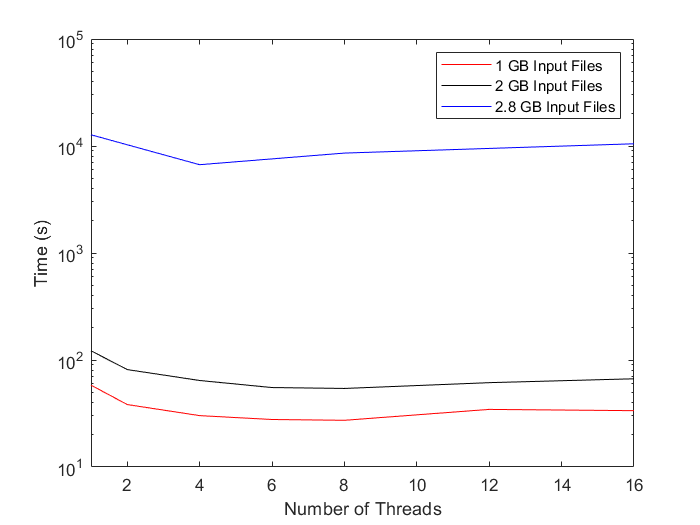
\includegraphics[width=1\columnwidth]{mapReduceTimevsThreads.png}
	\caption{Time taken for the equi-join vs number of threads for the MapReduce solution for various file sizes}
	\raggedright
	\label{fig:resultsMR}	
\end{figure}

\figref{fig:resultsMR} provides a graph of the time taken for the MapReduce equi-join per number of threads for the 1, 2 and 2.8GB input files. From the graph, it is clear that as the file size increases, the time to perform the join increases. It also indicates that for the smaller input files, the optimal performance is achieved for eight threads. However, for the large input file, the best performance is achieved when four threads are used. Since the node used to run the benchmarks had eight hardware threads, it is expected that running the program with eight threads would give the best performance. It is thus an outlier that the best performance for the 2.8GB input files was achieved for four threads. From the figure, it can also be inferred that when running the 2.8GB input file, all of the node's RAM was used, and as such, hard drive space was used for virtual memory \cite{ram}. Since hard drive I/O speed is much slower than RAM I/O speeds, the use of virtual memory results in the drastic speed decrease seen in the graph \cite{ram}.


\begin{figure}[h]
	\centering
	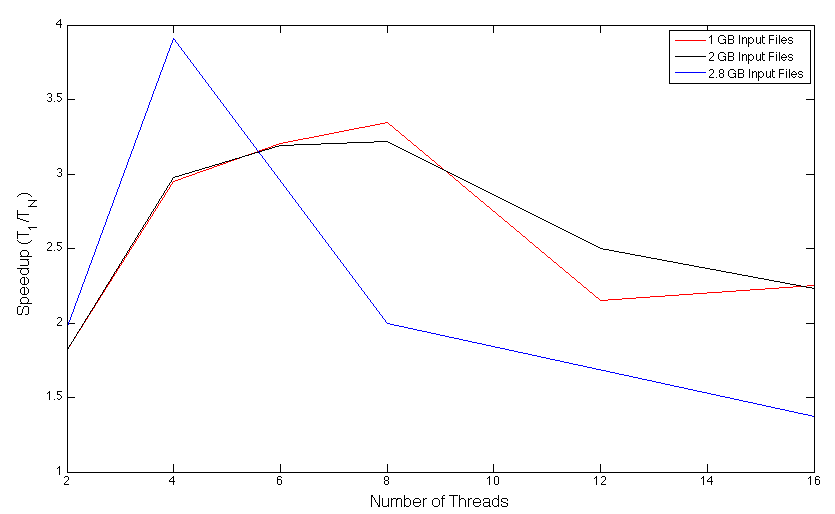
\includegraphics[width=1\columnwidth]{mapReduceSpeedup.png}
	\caption{Speedup plot for the MapReduce solution}
	\raggedright
	\label{fig:speedUpMR}	
\end{figure}

\figref{fig:speedUpMR} is a speedup plot for the MapReduce equi-join. Speedup is defined as the ratio of the execution time for one thread to that of N threads \cite{speedup}. The graph emphasises the conclusions made from \figref{fig:resultsMR}, being that as the number of threads increases, performance increases, until the maximum number of threads per core is exceeded. Thereafter, performance decreases.

A strength of the designed solutions is that both solutions are able to perform equi-join operations on any column of a table. Furthermore, the hybrid solution is able to handle any type of delimiter within a file.

\subsection{Limitations}
A limitation of the implemented MapReduce model is that an assumption is made that the reducer has sufficient memory to hold all of the values with the same key~\cite{mapReduceJoin}. If the reducer does not have sufficient memory, the performance of the algorithm is greatly affected.

\subsection{Tradeoffs} \label{sec:tradeoffs}
The use of a STL \texttt{std::vector} to store the hash join results is a large tradeoff of the system. While this usage allows for reduced computational complexity and improved platform compatibility, it creates redundancies in the efforts to parallelise all possible components of the hybrid equi-join algorithm. Therefore this design choice creates a large inefficiency within the system.

The use of memory mapping to store the input text files for the MapReduce solution is a large tradeoff of the system. While this usage means that larger input files can be processed, it also lead to the need to duplicate each input text file twice, and allocate memory for each of the four text files. This creates a large inefficiency within the system.

\section{FUTURE RECOMMENDATIONS}
For future recommendations, a hybrid hash-join algorithm should be implemented rather than a simple hash-join. This would improve performance at all levels of memory availability~\cite{evaluating4JoinAlgorithms}.

Furthermore, the performance of the hybrid equi-join algorithm could be greatly improved through the use of a concurrent vector, such as the Thread Building Blocks (TBB) \texttt{tbb::concurrent\_vector}, or by utilising the \texttt{std::mutex} class to manage thread synchronisation of modification operations to the STL \texttt{std::vector}~\cite{tbb,mutex}.

For future, each of the benchmarks run above should be repeated multiple times and the results should be averaged. This will allow for more accurate benchmarks to be acquired as it will minimise the effect of outliers in the results.

\section{CONCLUSION}
The design and implementation of two different equi-join algorithms were presented. The first was a hybrid model using MPI and OpenMP, that made use of a simple hash join to implement the equi-join. The second implemented the equi-join using the Phoenix++ MapReduce paradigm. Benchmarks were run by varying the input file size, along with the number of nodes and the number of threads being used by the two solutions. It was discovered that ?????????????. For future work, a concurrent vector should be used in the hybrid model to allow for parallel querying, thus drastically improving performance.

\bibliographystyle{witseie}
\bibliography{bigData}

\end{document}